\chapter{Statistics of Radioactive Decays}


\section{Introduction}

\begin{figure}[htbp]
\begin{center}
 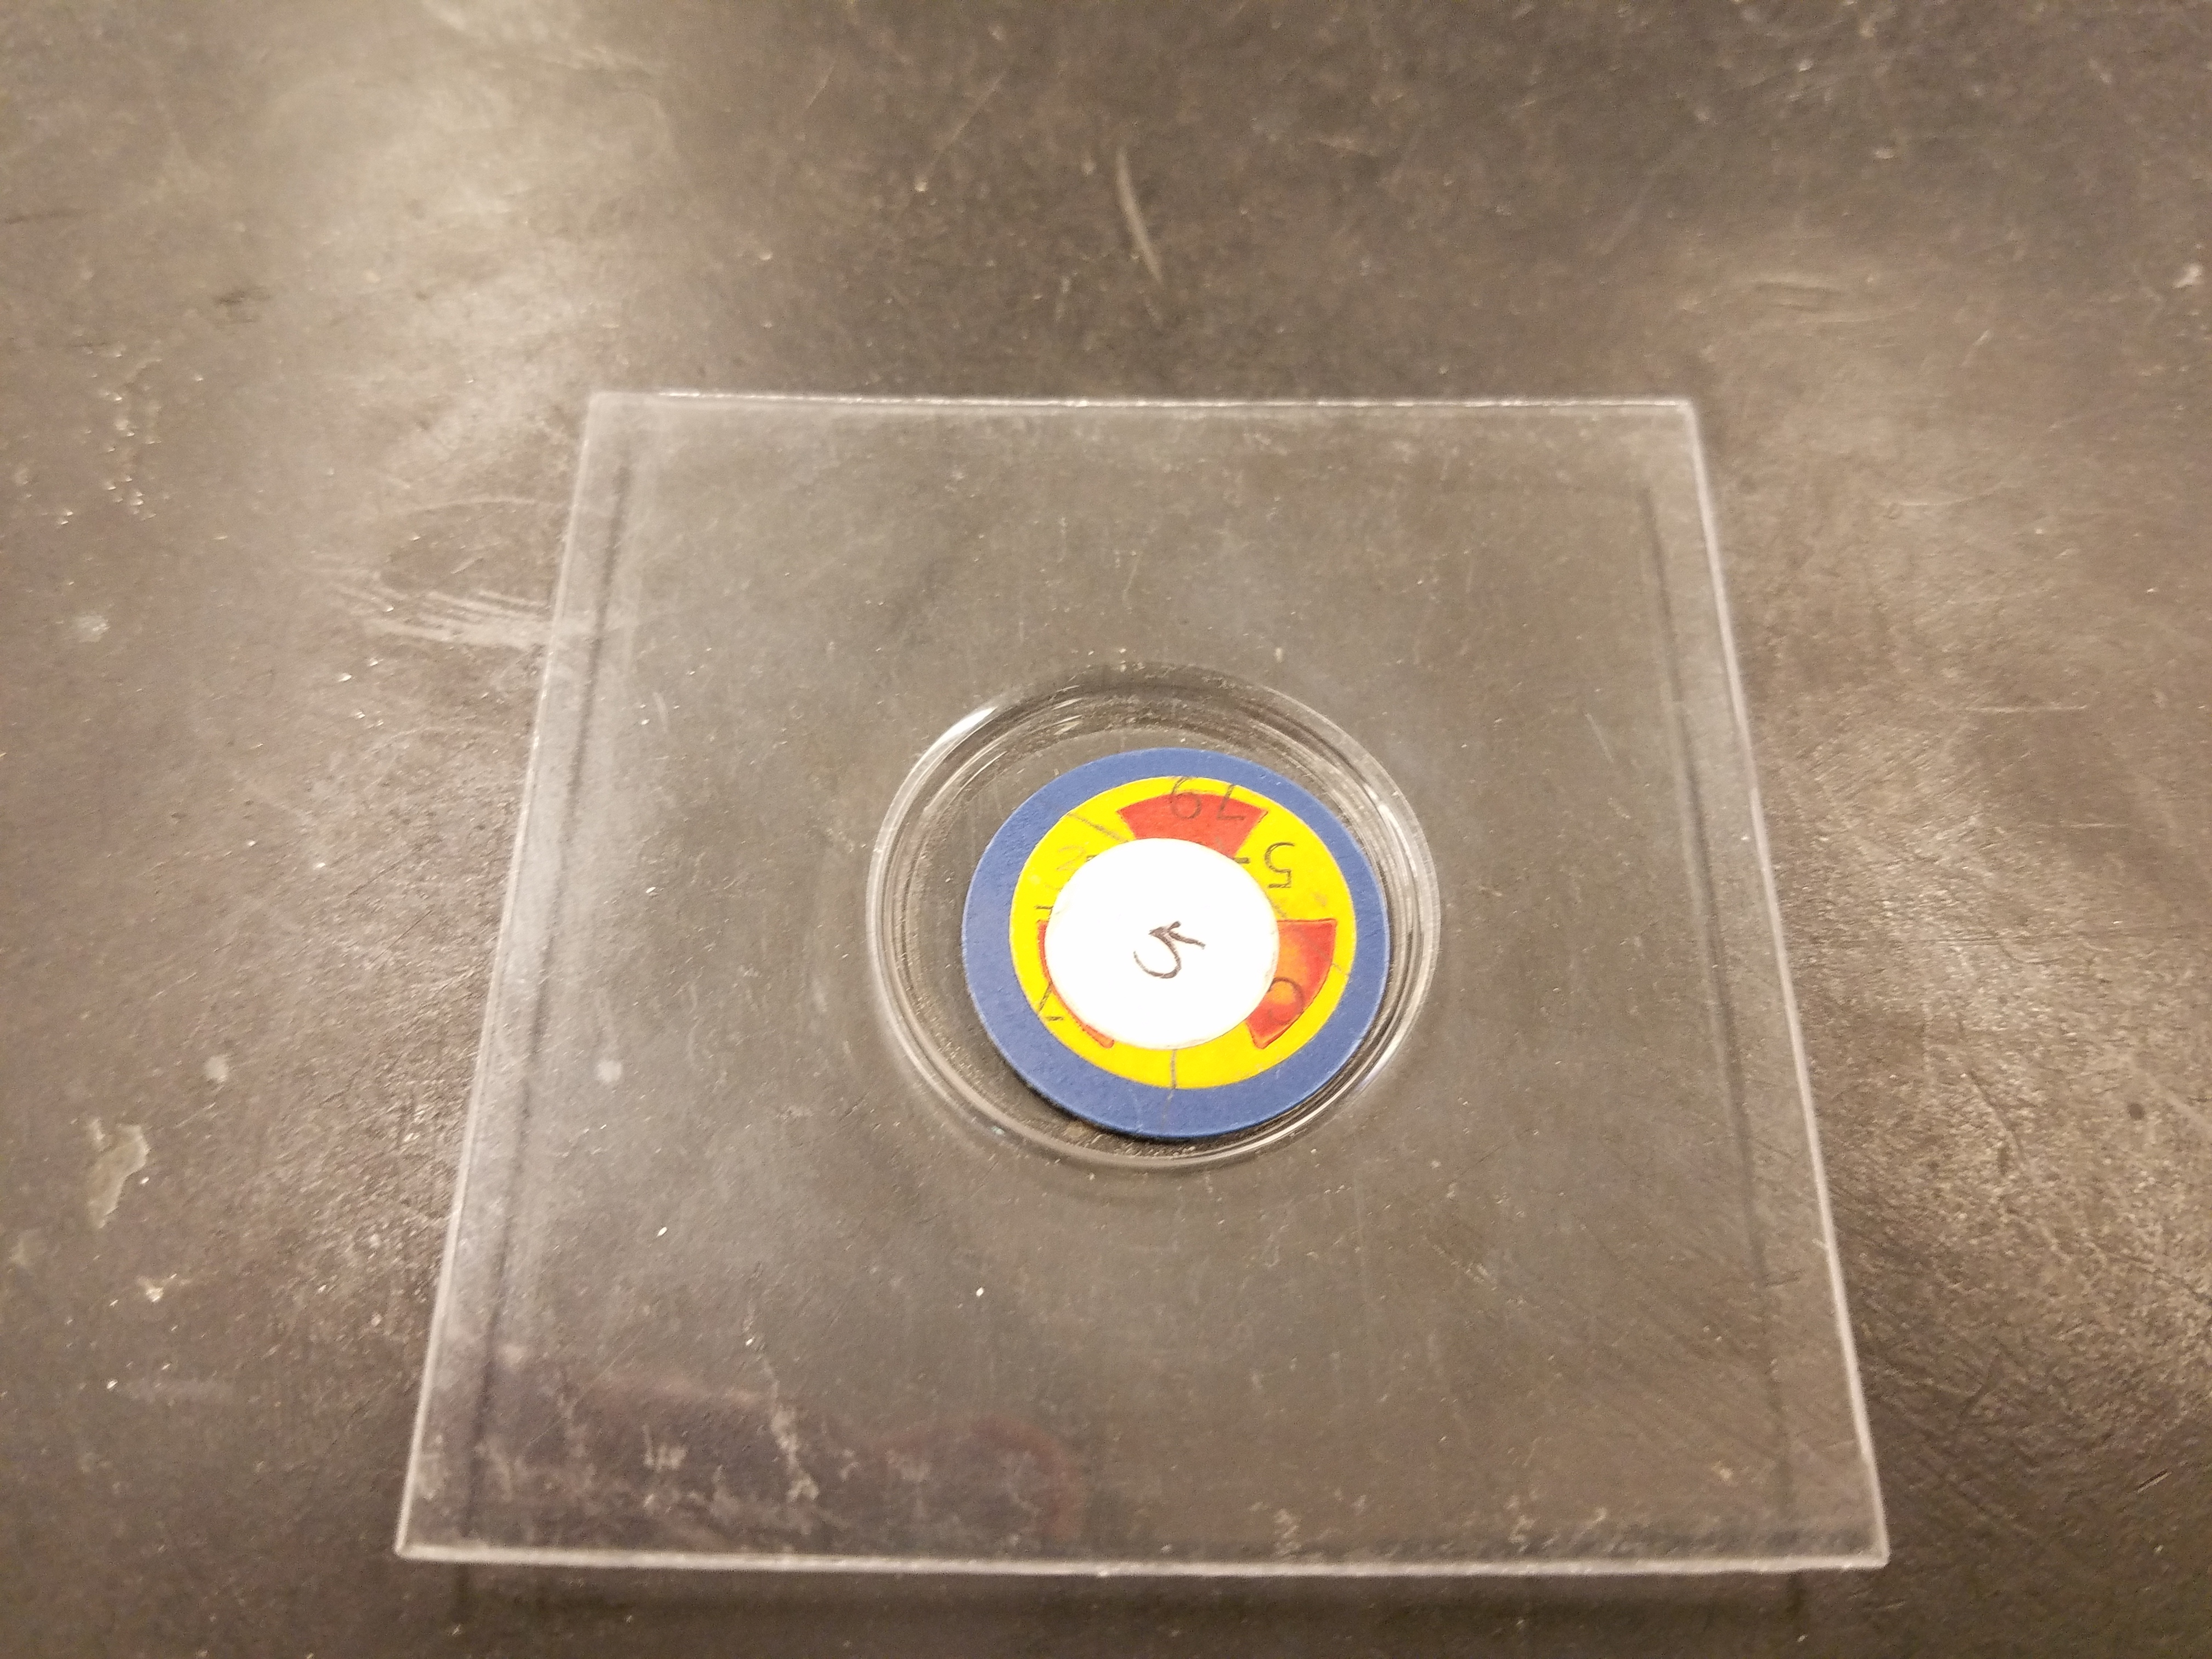
\includegraphics[width=0.55\textwidth]{figs/labs/geiger/source.jpg};
\caption{\label{fig:source} A sealed radioactive source.  A small
  amount of Cs-137 is contained within the small button shaped piece
  of plastic.  For your safety, the sources will be handled only by
  the TA.}
\end{center}
\end{figure}

In this lab, you will use a Geiger Counter to study the statistics of
radioactive decays.  For this lab there are both logbook and Jupyter
notebook entries.

\section{Precautions}

\noindent
{\bf Precautions with the Geiger counter:}
\begin{itemize}
\item Leave the cable from the Geiger counter controller to the Geiger
  counter in place {\em at all times}.  This carries voltages of
  approximately 1000 volts.  If you leave the cable in place, nothing
  can be inadvertently plugged in (including fingers).
\item Leave the Geiger tube in its holder.  It has a thin front window
  which is easily broken.
\item Do not set the high voltage higher than 1000 volts.
\end{itemize}

\noindent
{\bf Precautions with the radioactive source:}
\begin{itemize}
\item See Fig.~\ref{fig:source} to familiarize yourself with what the sources look like.
\item Don't touch the source.
\item Leave the source in the tray at all times.  The TA will provide
  the sources and handle moving them from place to place.
\item Radiation falls off as $1/r^2$.  So minimize your time near
  sources and maximize your distance from them.
\end{itemize}

\section{The Geiger Counter}

\begin{figure}[htbp]
\begin{center}
\begin{tikzpicture}
    \node[anchor=south west,inner sep=0] (image) at (0,0,0) {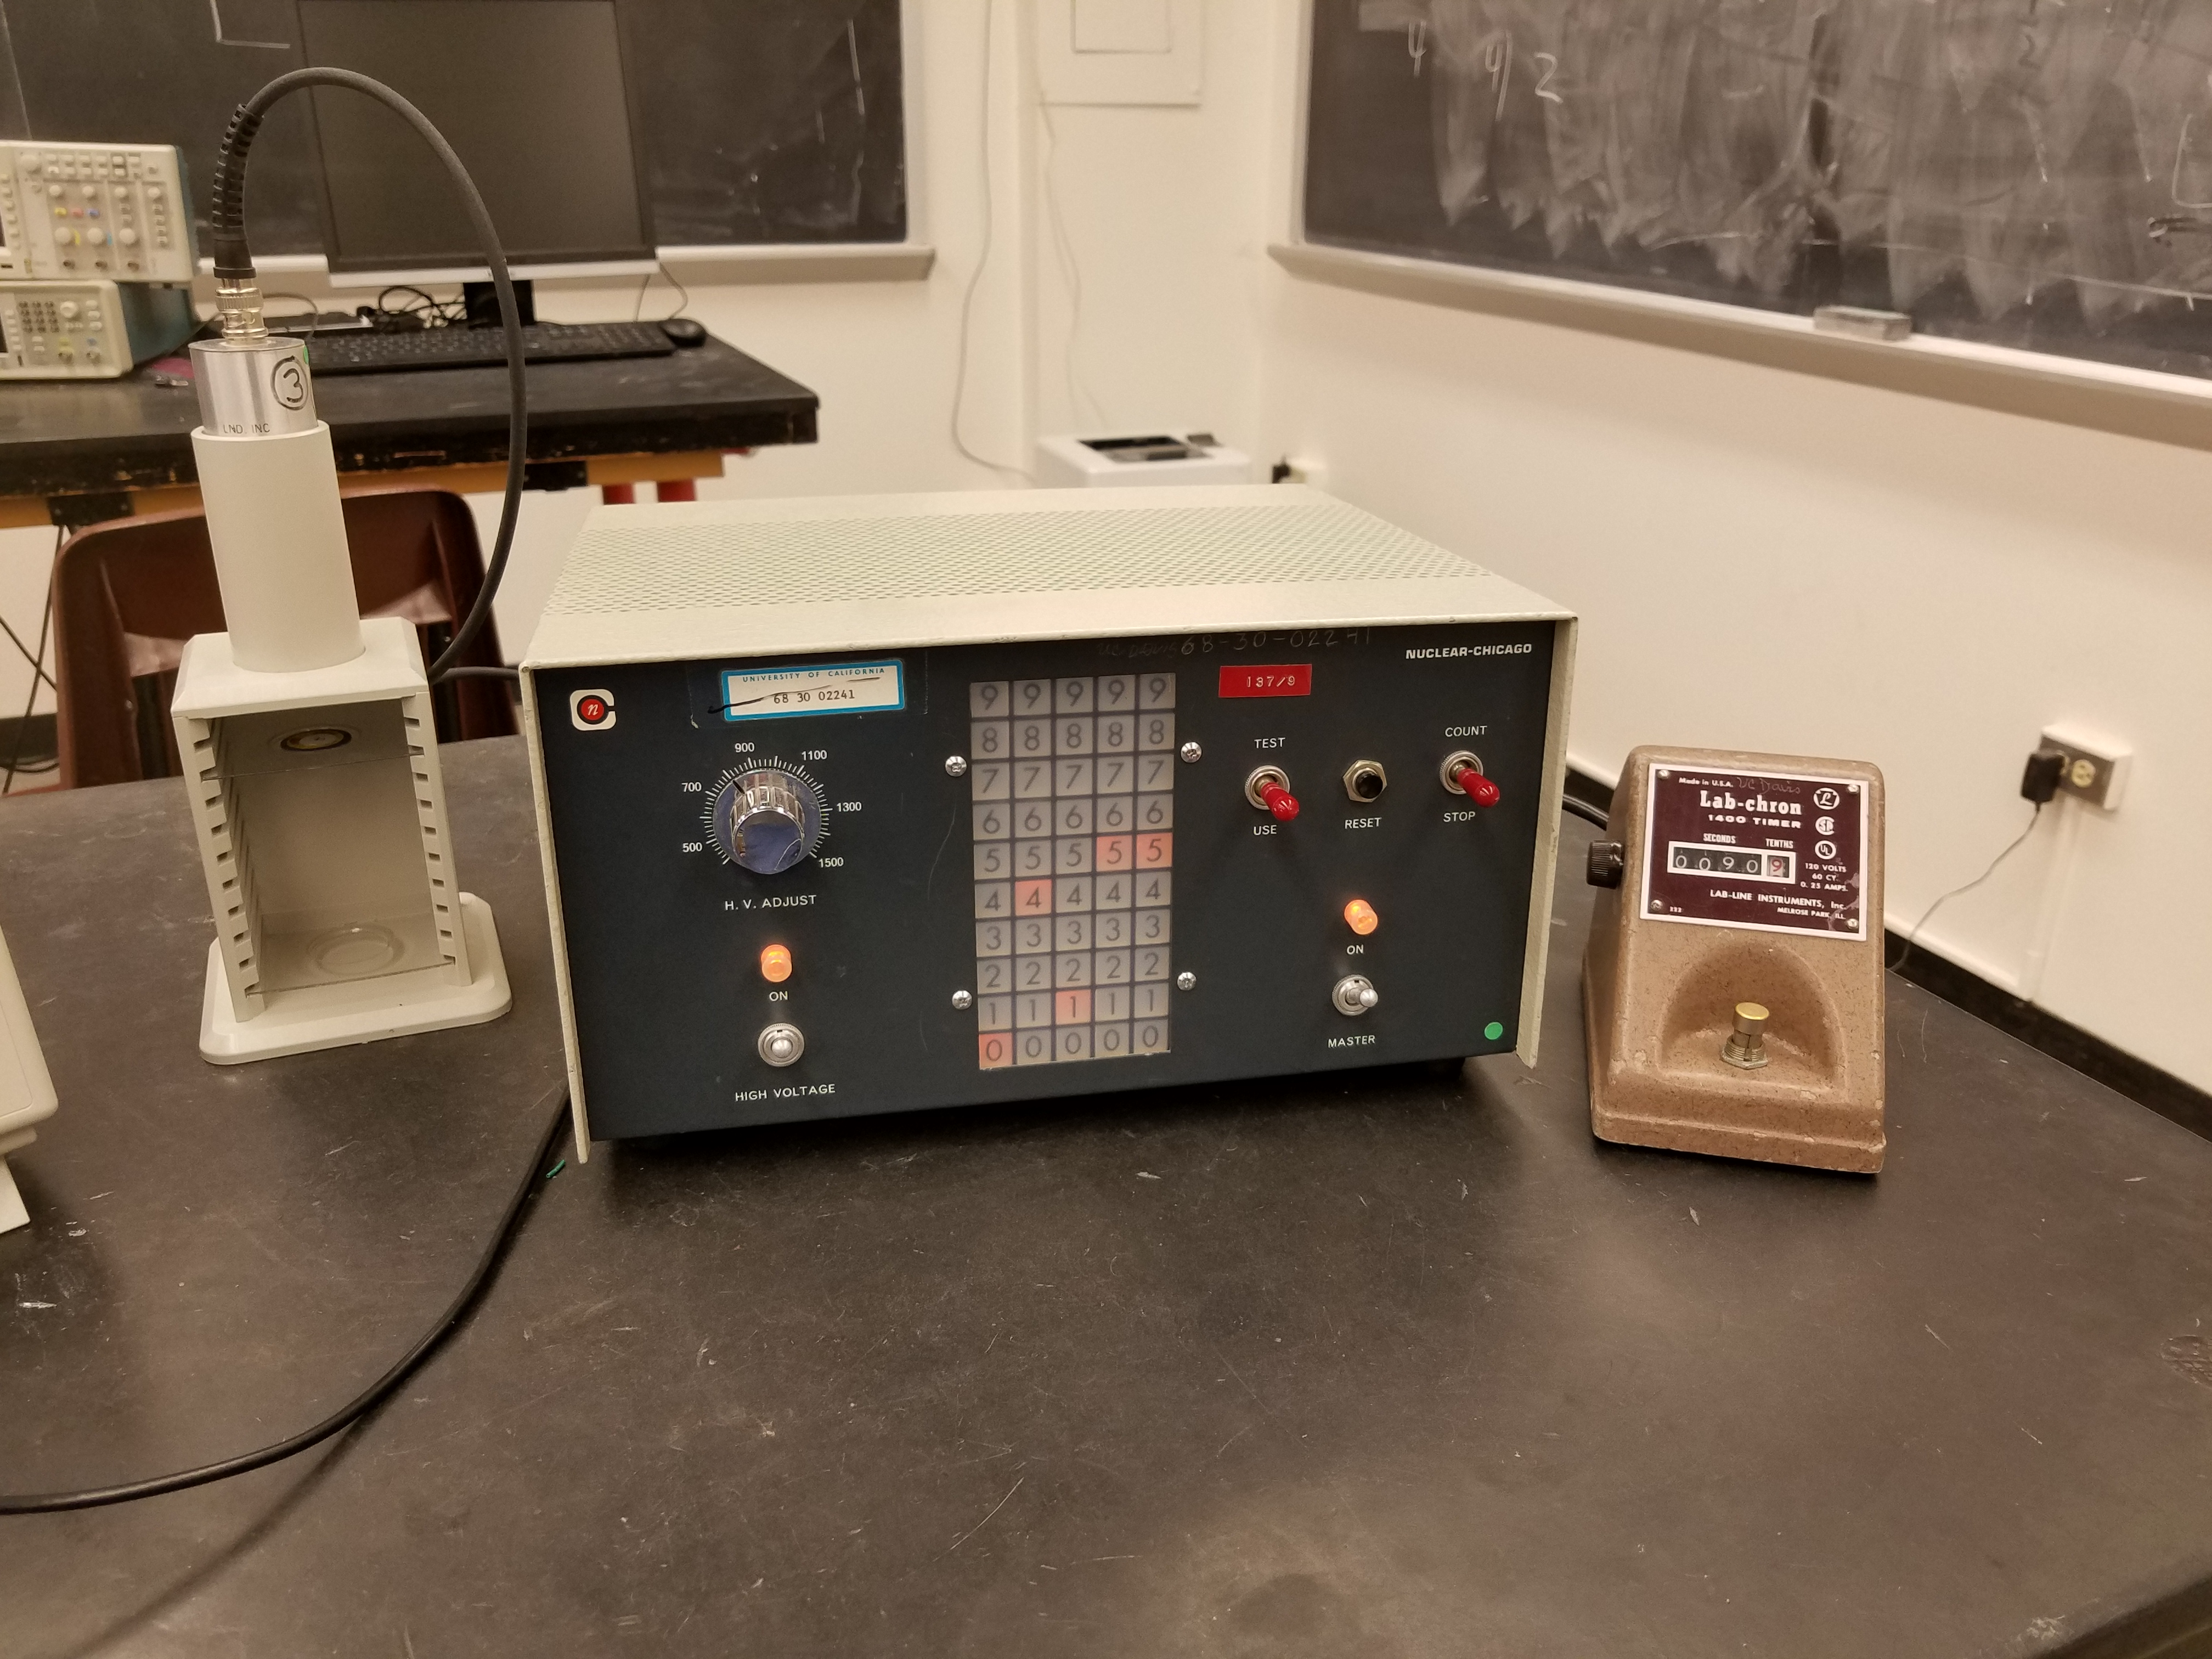
\includegraphics[width=0.55\textwidth]{figs/labs/geiger/assembly.jpg}};

    \node[right](X) at (10.0,3.0) {Timer};
    \draw (X.west) -- (8.0,3.5);

    \node[right](X) at (10.0,5.0) {\parbox{3cm}{\flushleft High-Voltage and Counter}};
    \draw (X.west) -- (5.0,4.75);

    \node[left](X) at (0.0,4.5) {\parbox{2.5cm}{\flushright Geiger Tube Holder}};
    \draw[white,thick] (X.east) -- (1.25,5.0);
    \draw (X.east) -- (1.25,5.0);

    \node[left](X) at (0.0,3.0) {Source};
    \draw (X.east) -- (1.35,4.05);

\end{tikzpicture}
\caption{\label{fig:geigersetup} The Geiger Counter assembly.}
\end{center}
\end{figure}

To begin, familiarize yourself with the counter and timer features of
your Geiger counter assembly using the built-in test mode.  Your lab
bench will already be prepared with a Geiger Counter assembly as shown
in Fig.~\ref{fig:geigersetup}.  Ensure that the high-voltage (HV) is
off by turning the knob labeled ``H.V. Adjust'' counter-clockwise all
the way to zero.  Now put the Geiger counter into test mode by
flipping the left red switch to ``TEST''.  Flip the right red switch
to ``COUNT'' and you should see the counter display begin
incrementing.  Push the button on the front of your timer and you
should see the Timer turn on and off.  Leave the timer incrementing.
Now flip right red switch to ``STOP'', and observe that the both the
counter and the timer stop simultaneously.  The knob on left side of
the old-school lab timer can be used to reset the time.  Keep turning
the knob clockwise until the time reads 0.  Use the black button on
the Counter to reset the count to zero.

Flip the right switch to ``COUNT'' and then back to ``STOP'' when 10
seconds have passed.  During this time, the $60~\rm Hz$ test signal
should increment the counter close to 600 times.  Try this a few times
and make sure you can reliably count close to $600$ test pulses in a
10 second interval.  You should reset the count each time, but there
is no need to reset the timer.  Simply stop when the timer reaches the
next factor of ten.  Due to your reaction time, you may well stop at
one-to-two tenths of a second later.  This is OK, and will only add
less than a few percent error to your measurements over 10 second
intervals.

\section{High-Voltage Calibration}

When you are confident that you know how to operate the timer, switch
the left red switch to ``USE'' mode.  Unless a sealed radioactive
source is already in place, ask the TA to provide you with a source in
the second shelf from the top of your Geiger tube holder.  Switch the
right switch to ``COUNT'' mode.  With the HV off, you should not see
any pulses.  Turn the HV up until you begin to see counts increment on
the display, and continue to the next interval of 50 volts (e.g. if it
first starts incrementing at 730 volts, set the dial to 750 volts).
Count the number of events in a ten second interval.

Repeat this measurement in 50 volt steps up to 1000 volts.  Do not exceed 1000 volts.

\begin{plot}
Plot the rate (in Hz) as a function of high voltage.  You should see a
plateau region (a leveling off) which indicates the onset of the
Geiger mode within the Geiger tube.  The Geiger tube has some
resistance even in Geiger mode, so do not expect a perfectly flat
plateau.  From your plot, chose a high-voltage near the beginning of
the Geiger mode, and set the high-voltage to this calibrated value.
If you are struggling with Python, you can make a rough plot by hand
in your logbook to determine the plateau region, and leave the fancy
plot for later.
\end{plot}

\begin{figure}[htbp]
\begin{center}
 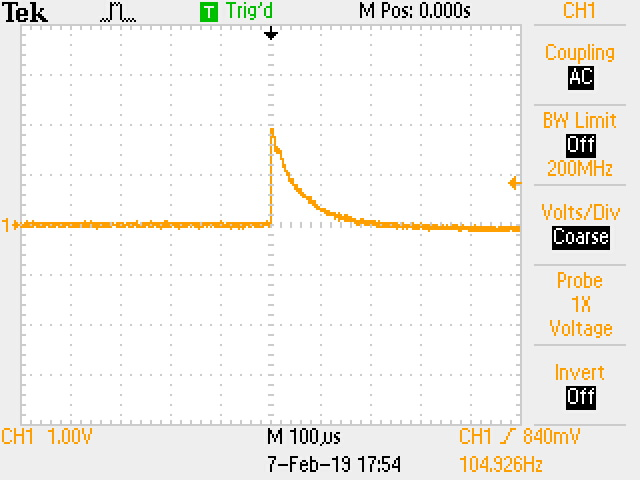
\includegraphics[width=0.55\textwidth]{figs/labs/geiger/pulse.jpg};
\caption{\label{fig:geigerpulse} An example Geiger counter pulse.}
\end{center}
\end{figure}

Connect an oscilloscope to the output of the counter assembly (on the
back, labeled ``SCOPE'').  Adjust your scope to view the Geiger pulses
like that of Fig.~\ref{fig:geigerpulse}.  Note that the Geiger counter
output contains a DC component in addition to the AC pulse, so you
will want to use your scope in AC coupling mode which will remove the
DC component and allow you to see the pulse.  You will also want to
see the attenuation to 1X because you are not using an attenuating
probe.

\begin{measurement}
Sketch a typical Geiger counter pulse in your logbook and indicates the pulse height and time duration.
\end{measurement}

\section{Data Collection}

Even in today's world of digital automation, it is still useful to
know how to collect a small amount (up to a few hundred data points)
of data manually.  Often in the lab, you have one-off measurements
that you would like to make without investing in automation.

In this section, you will collect data manually for about one hour.
Practice a routine with your lab partner that allows you to take and
record the data as fast as possible.  For instance, person A should
operate the counter, and person B should use the PC.  Person A turns
the counter on for ten seconds, turns it off, and says (quietly)
``OK''.  Person B records the value on the PC and says ``Go''.  Person
A resets the counter and continues.  Remember that there is no need to
reset the Timer each time, which would take too long, and which would
actually be counterproductive (if you consider the effect of a roughly
constant reaction time.) 

Practice your routine a few times, and make sure your count is near
1000 events in a ten second interval.  Then record 120 data points.

When you have finished recording your data with the radioactive
source, ask your TA to remove the source and return it to the
radioactive locker.

Now record an additional 120 data points with no source, to measure
the background radiation rate.  You should record around 3 background
counts per 10 second interval.

\section{Analysis}

\begin{figure}[htbp]
\begin{center}
\begin{tabular}{cc}
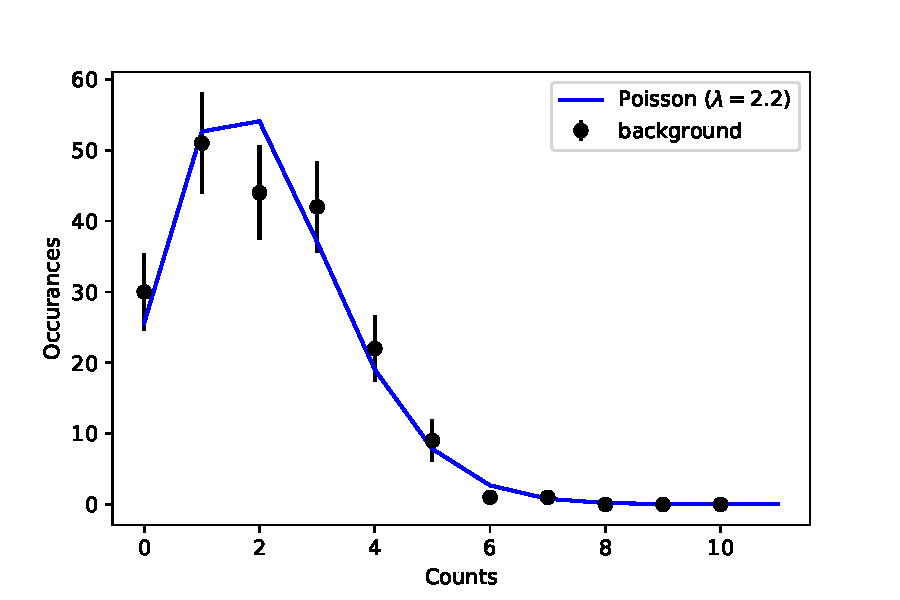
\includegraphics[height=0.22\textheight]{figs/labs/geiger/background.pdf}
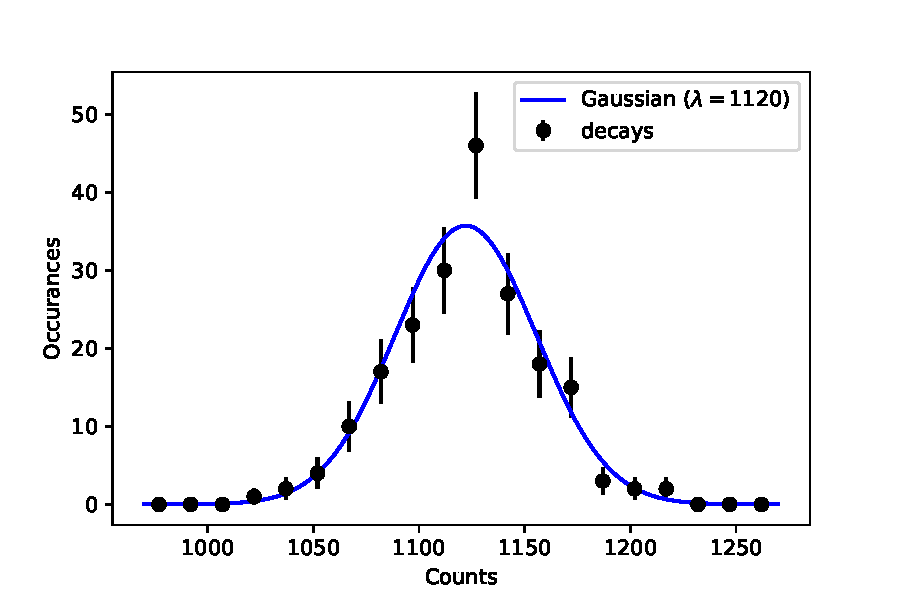
\includegraphics[height=0.22\textheight]{figs/labs/geiger/source.pdf}
\end{tabular}
\end{center}
\caption{\label{fig:geigeranalysis} Numerical simulation of the experiment
  for (a) background radiation only, and (b) radioactive source
  present.}
\end{figure}

Using Scientific Python, measure the mean and variance of your
collected background and source data.  Then produce histograms to
display your data as in Fig.~\ref{fig:geigeranalysis}.  For the
background data, plot the histogram for eleven bins: 0,1,2,...,10.
For the source data, plot about 20 bins covering a few hundred counts
around the mean value.

\begin{plot} Compare your collected background data to a Poisson distribution,
appropriately normalized, with a mean set to the mean of your data. \end{plot}
\begin{plot} Compare your collected source data to a Gaussian distribution,
appropriately normalized, with a mean set to the mean value of your
data, and sigma set to the square root of your mean. \end{plot}

This is a \textbf{sign-off point} for this lab. 
%move this earlier have them take data with source and analyze then sign off point plus data taking for only background plus analysis; so if they are late they get some plots that could be discussed.








